% Define table for personas.
\newcommand{\persona}[4]{%
    \textbf{#1}
    \small\begin{tabular}[t]{|p{.8in} | p{1.5in}|}
        \hline
        \textbf{Preferences} & #2 \\\hline
        \textbf{Pain Points} & #3 \\\hline
        \textbf{Goals} & #4 \\
        \hline
    \end{tabular}
    \vspace{4pt}
}


\chapter{Introduction}
\label{chap:introduction}

\section{Background}
\label{section:background}

In large campus and factory environments, tracking people across multiple cameras is crucial for safety, security, and operational efficiency. Security teams need to quickly locate individuals involved in incidents like theft or unauthorized access. Factory managers require clear understanding of worker movements to ensure safety protocol compliance. Emergency responders need to pinpoint locations during evacuations. Without effective multi-camera tracking, blind spots and identification failures lead to delayed responses and compromised safety \cite{wangetal:2021}.
When individuals transition between camera views, maintaining their identity becomes challenging. Existing systems often fail during these handoffs, creating fragmented surveillance coverage. For example, a student moving from an outdoor courtyard to a building lobby might be lost during transition, making it difficult to determine if they later entered a restricted area. This problem is particularly significant in sprawling campuses with numerous buildings or complex factory layouts where cameras operate independently.
Environmental factors further complicate tracking. Lighting differences between bright outdoor areas and dim hallways alter appearances significantly. Crowded periods during class changes or shift rotations create frequent occlusions. Cameras at varying heights and angles provide drastically different perspectives of the same person, hindering accurate matching across views - a bag visible from the side might be completely hidden from the front.
Our project aims to develop a robust tracking system called \textit{SpotOn} that consistently identifies and tracks individuals across camera networks, providing uninterrupted coverage in campus and factory settings. By solving the identity maintenance challenge across camera transitions, our solution will enhance security monitoring, expedite emergency responses, and provide valuable data for facility management and resource optimization.

\section{Problem Statement}
\label{section:problem-statement}

The problem statement for the \usevar{\srsTitle} addresses the fundamental challenge of maintaining consistent identification of individuals as they move through spaces monitored by multiple cameras. In various environments from campuses and factories to public spaces and transportation hubs, the ability to track individuals across camera transitions is critical yet remains largely unsolved. When a person moves from one camera's view to another, current systems frequently lose their identity trail, creating fragmented tracking data that fails during situations requiring continuous monitoring. This tracking discontinuity affects numerous applications—from security monitoring and emergency response to space utilization analysis and research on movement patterns. The consequences include critical delays during time-sensitive situations, incomplete data for operational decision-making, and increased workload for monitoring personnel who must manually reconnect identity fragments across camera boundaries.
Technically, this challenge manifests in three interconnected problems. First, the multi-view detection problem requires accurately identifying and locating individuals within each camera feed despite visual challenges like occlusions, distance variations, and diverse human appearances across different environments. Second, the cross-camera identity preservation problem involves maintaining consistent person identification during transitions between non-overlapping camera views, where individuals may appear drastically different due to perspective shifts, lighting changes, and temporal gaps. Third, the unified spatial comprehension problem necessitates integrating observations from distributed cameras into a coherent coordinate framework that enables operators to visualize continuous trajectories and understand movement patterns throughout the entire monitored environment. Current systems address these problems in isolation rather than as an integrated challenge, resulting in fragmented surveillance coverage that fails during critical monitoring scenarios.


\section{Solution Overview}
\label{section:solution-overview}

The \usevar{\srsTitle} addresses multi-camera person tracking challenges through an integrated computer vision platform with three core technical components:

\subsection{Prominent Features}
\label{subsection:main-features}

\begin{enumerate}[leftmargin=80pt]
    \item \textbf{Multi-View Person Detection:} A system that identifies and locates all individuals within each camera feed, creating bounding boxes around people in the video frames. This detection works independently on each camera, handling challenges like partial occlusions, varying lighting conditions, and environmental changes without attempting to match identities across cameras.

    \item \textbf{Cross-Camera Re-Identification and Tracking:} A specialized system that matches and tracks individuals across different camera views. When someone exits one camera's view and appears in another camera, this system maintains their identity by analyzing visual features like clothing, size, and walking patterns. The tracking component continuously updates each person's position and trajectory, preserving their identity across camera transitions despite changes in perspective, lighting, and viewing angle.

    \item \textbf{Unified Spatial Mapping:} A mapping system that transforms detections from distributed cameras into a coherent coordinate system. This integration enables continuous trajectory visualization as individuals move through the monitored environment across multiple camera views, providing operators with a comprehensive spatial understanding of movement patterns throughout the facility.
\end{enumerate}

\subsection{Optional Features}
\label{subsection:optional-features}

\begin{enumerate}[leftmargin=80pt]
    \item \textbf{LLM-Powered Person Selection:} A natural language interface that allows users to identify individuals based on descriptive prompts (e.g., "Find the person wearing a black jacket and jeans who passed through the main entrance at 2:30 PM"), with an interactive confirmation step where users select the correct person from highlighted candidates.

    \item \textbf{Multi-Person Tracking:} Capability to simultaneously maintain identity and location data for multiple individuals across the camera network, preserving each person's unique identity despite occlusions, varying viewing angles, or extended periods where individuals are not visible in any camera.

    \item \textbf{Movement Pattern Analysis:} AI-powered analysis to identify typical movement patterns and provide insights for space utilization, traffic management, and anomaly detection in pedestrian flows across the monitored environment.

    \item \textbf{Configurable Model Parameters:}  A settings interface enabling users to fine-tune system performance by adjusting core parameters, including detection confidence, processing framerate, bounding box appearance, and Intersection over Union (IOU) threshold for object matching. This allows adaptation to specific environmental conditions and computational resources.
    
    \item \textbf{Environmental Analytics Dashboard:} Real-time metrics including occupancy density maps, path trajectory analysis, and movement pattern heatmaps tailored for facility management, safety monitoring, and resource optimization.
\end{enumerate}

\subsection{Stretch Goals}
\label{subsection:stretch-goals}

\begin{enumerate}[leftmargin=80pt]
    \item \textbf{Voice Command Integration:} Allow personnel to interact with the system using natural voice commands (e.g., "Track the person in the blue jacket heading toward Building B") for hands-free operation during critical situations.

    \item \textbf{Anomaly Detection:} Implement AI-powered anomaly detection to automatically identify unusual behavior patterns (such as suspicious movements, crowd formations, or potential security incidents) across the monitored environment.

    \item \textbf{Privacy-Preserving Tracking:} Implement anonymization techniques that maintain tracking capabilities while protecting individual privacy through face blurring or feature abstraction in accordance with surveillance regulations and privacy laws.

    \item \textbf{Automatic Environment Mapping:} System that creates spatial representations based on observed movement patterns, automatically identifying walkways, intersections, and common routes without requiring manual mapping of the environment.
\end{enumerate}

\section{Target User}
\label{section:target-user}

The \usevar{\srsTitle} enables professionals in security, facility management, and emergency response to maintain consistent identification of individuals across multiple camera views in complex environments, enhancing safety, optimizing operations, and improving response times.
The primary users are personnel responsible for monitoring distributed camera networks across large spaces.

\begin{table}[p]
    \centering
    \noindent\begin{tabular}{| p{2.65in} | p{2.65in} |}
        \hline & \\[-10pt]
        \persona{Security Officer}
        {Track subjects across non-overlapping camera zones, identify unauthorized access.}
        {Loses identity between cameras, spends critical time searching feeds during incidents.}
        {Maintain continuous tracking, quickly locate persons of interest, coordinate response teams.} &
        \persona{Facility Manager}
        {Monitor space utilization, analyze traffic patterns, plan resource allocation.}
        {Cannot capture comprehensive movement data for occupancy planning or identify bottlenecks.}
        {Optimize space usage, identify congestion points, make data-driven facility decisions.} \\[10pt]
        \hline & \\[-10pt]
        \persona{Emergency Coordinator}
        {Track evacuations, monitor crowd density, coordinate personnel during incidents.}
        {Lacks complete situational awareness across transition zones between cameras.}
        {Ensure safety compliance, rapidly locate individuals needing assistance, coordinate resources.} &
        \persona{Analytics Specialist}
        {Extract behavioral insights, analyze movement patterns, develop predictive models.}
        {Cannot integrate cross-camera data for comprehensive movement analysis.}
        {Identify usage trends, measure operational efficiency, provide data-backed improvement recommendations.} \\[10pt]
        \hline
    \end{tabular}
    \caption{Personas from User Analysis for \usevar{\srsTitle}}
\end{table}

\newpage

\section{Benefit}
\label{section:benefit}
The \usevar{\srsTitle} delivers benefits directly addressing the three key challenges in multi-camera tracking. The multi-view person detection with environmental adaptation ensures reliable tracking despite lighting changes, occlusions, and perspective differences.
The cross-camera re-identification solves the identity preservation problem by maintaining continuous tracking between cameras, eliminating fragmentation when individuals move through non-overlapping camera networks.
The unified spatial mapping creates a comprehensive environmental understanding by integrating all camera feeds into a single coordinate system, allowing operators to visualize movement patterns spanning multiple buildings and zones.
These capabilities translate to 70\% reduced manual tracking workload, faster incident response times, more effective resource allocation, and comprehensive situational awareness across the entire monitored environment.

\section{Timeline}
\label{section:timeline}

\begin{figure}[!htb]
    \centering
    \makebox[\textwidth][c]{
        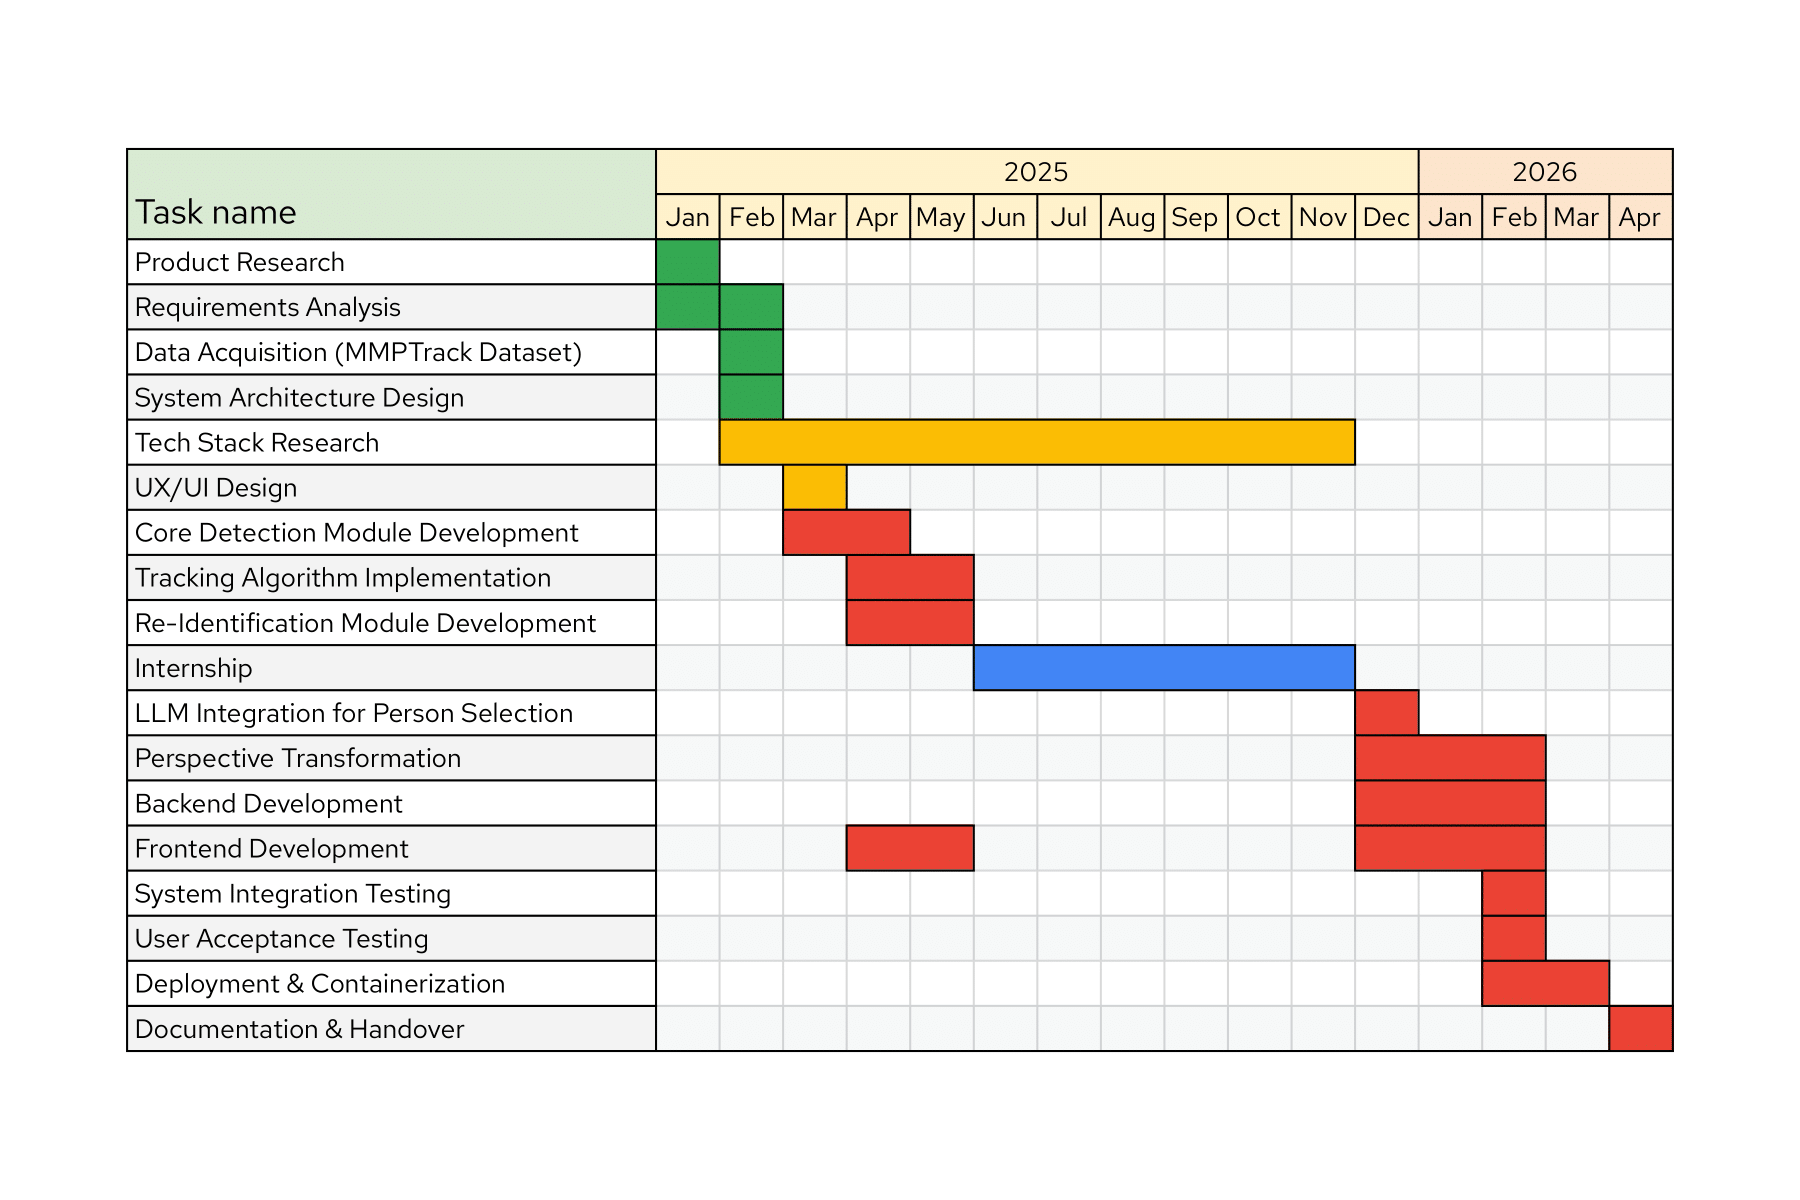
\includegraphics[width=1.2\textwidth,height=1.2\textheight,keepaspectratio]{jubjones/timeline.png}
    }
    \caption{Timeline for \usevar{\srsTitle}}
    \label{fig:timeline}
\end{figure}
\clearpage
As shown in figure \ref{fig:timeline}, it represents the timeline of the project.
The project began with product research in January 2025, followed by requirements analysis spanning January to February 2025. Data acquisition using the MMPTrack Dataset and system architecture design were completed in February 2025.

Technical stack research extended from February to November 2025, while UX/UI design was completed in March 2025. Core detection module development occurred in March-April 2025, with tracking algorithm implementation and re-identification module development taking place from April to May 2025.

An internship period ran from June to November 2025. LLM integration for person selection was completed in December 2025, while perspective transformation, backend development, and frontend development all occurred from December 2025 to February 2026.

System integration testing and user acceptance testing were conducted in February 2026. Deployment and containerization followed from February to March 2026, with final documentation and handover scheduled for completion in April 2026.


\section{Terminology}
\label{section:terminology}

\begin{itemize}[leftmargin=40pt]
    \item \textbf{\textit{Object Detection}}---a computer vision technique that identifies and locates objects within digital images or video frames, serving as the foundation for tracking individuals in each camera view.
    \item \textbf{\textit{Re-Identification (Re-ID)}}---the process of matching individuals across different camera views by comparing appearance features, enabling consistent identity preservation as people move between cameras.
    \item \textbf{\textit{Multi-Target Multi-Camera Tracking (MTMCT)}}---the task of tracking multiple individuals across a network of cameras with non-overlapping fields of view, maintaining identity consistency despite spatial and temporal gaps.
    \item \textbf{\textit{Feature Extraction}}---the process of identifying distinctive visual characteristics from a person's image that remain consistent despite environmental variations, critical for successful re-identification.
    \item \textbf{\textit{Spatial Mapping}}---a technique that converts observations from multiple camera views into a unified coordinate system, enabling continuous trajectory visualization across the entire monitored environment.
    \item \textbf{\textit{Occlusion Handling}}---methods to maintain tracking when individuals are partially or temporarily hidden by objects, structures, or other people in the camera view.
\end{itemize}